\setkeys{Gin}{width=0.7\textwidth}
\section{Results}\label{sec:results}
Four circuits were assembled and analyzed using a function generator to apply a stimulus sinusoid of 1\si{\voltpp} at 1\si{\kilo\hertz}, and an oscilloscope to measure the output of the system. Circuit schematics are taken from the lab manual \cite{lab-manual}.

\begin{figure}[htbp]
	\centering
	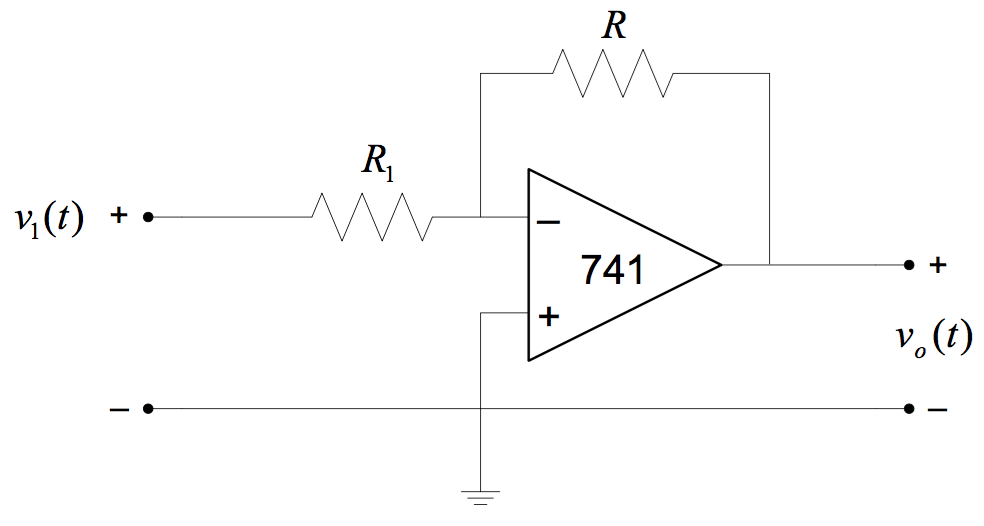
\includegraphics{schematic-inverter}
	\label{fig:schem-inverter}
	\caption{Inverter circuit schematic: $R_1=R=10\si{\kilo\ohm}$}
\end{figure}
\begin{figure}[htbp]
	\centering
	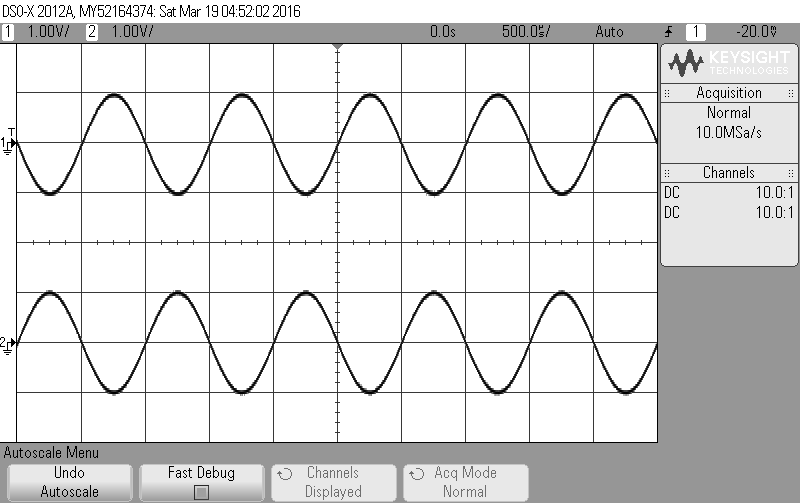
\includegraphics{response-inverter}
	\label{fig:inverter}
	\caption{Input and output of inverter circuit}
\end{figure}

\begin{figure}[htbp]
	\centering
	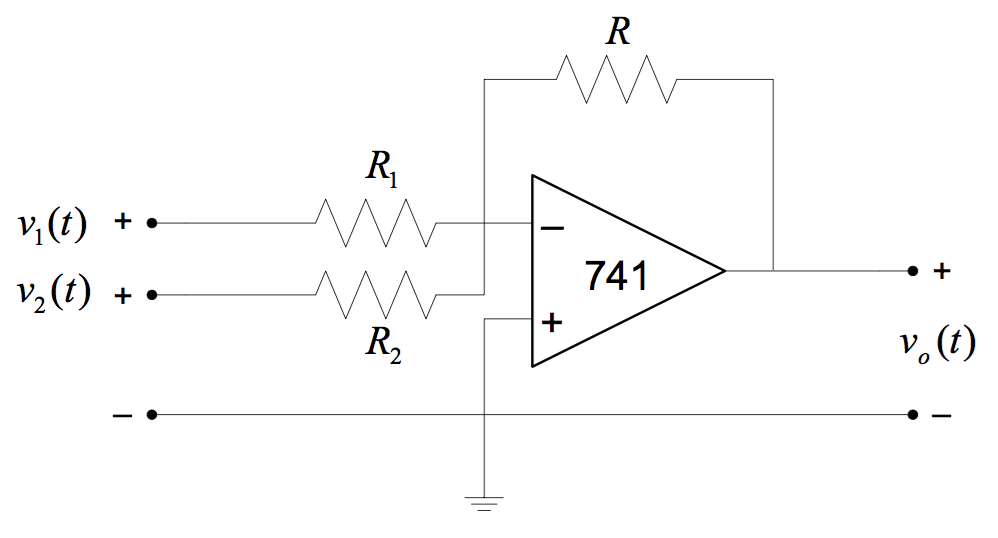
\includegraphics{schematic-adder}
	\label{fig:schem-adder}
	\caption{Adder circuit schematic: $R=R_1=R_2=10\si{\kilo\ohm}$}
\end{figure}
\begin{figure}[htbp]
	\centering
	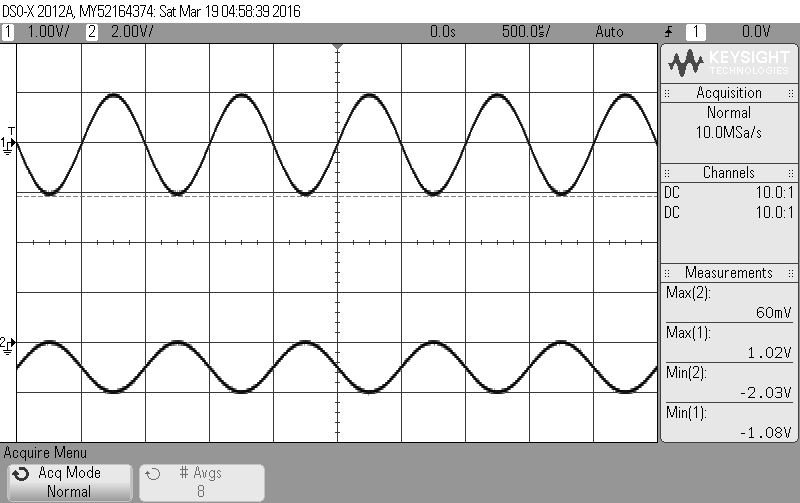
\includegraphics{response-adder}
	\label{fig:adder}
	\caption{Input and output of adder circuit}
\end{figure}

\begin{figure}[htbp]
	\centering
	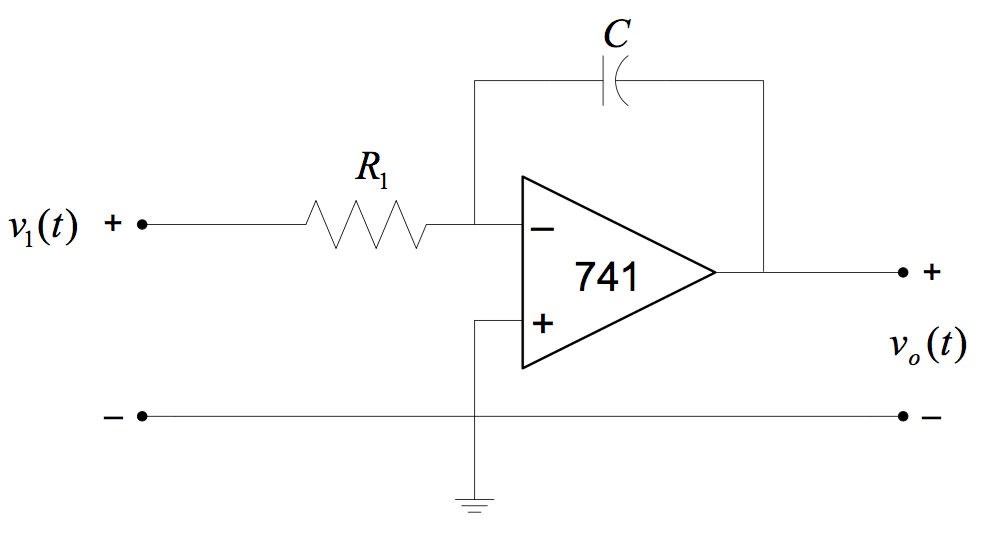
\includegraphics{schematic-integrator}
	\label{fig:schem-integrator}
	\caption{Integrator circuit schematic: $C=16\si{\nano\farad}$, $R_1=10\si{\kilo\ohm}$}
\end{figure}
\begin{figure}[htbp]
	\centering
	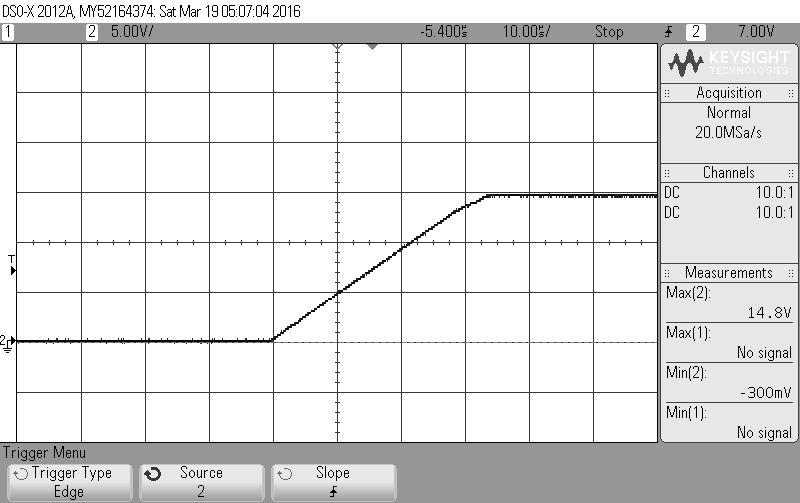
\includegraphics{response-integrator}
	\label{fig:integrator}
	\caption{Input and output of integrator circuit}
\end{figure}

\begin{figure}[htbp]
	\centering
	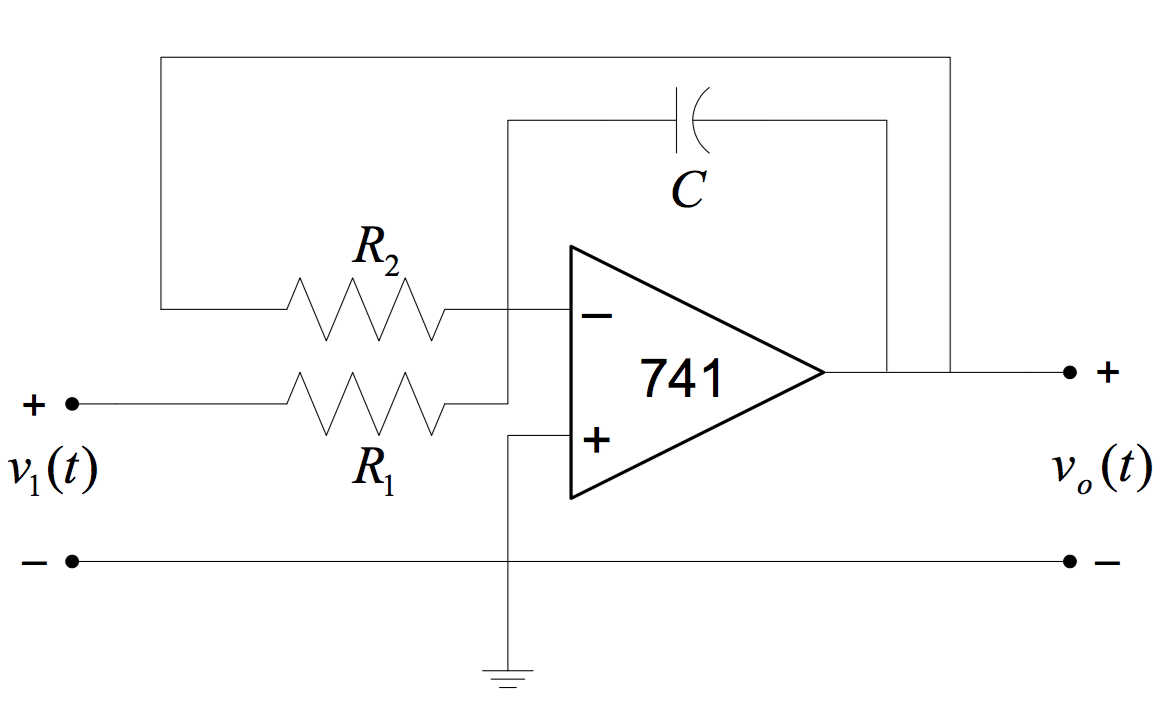
\includegraphics{schematic-first-order}
	\label{fig:schem-first-order}
	\caption{First order circuit schematic: $C=16\si{\nano\farad}$, $R_1=R_2=10\si{\kilo\ohm}$}
\end{figure}
\begin{figure}
	\centering
	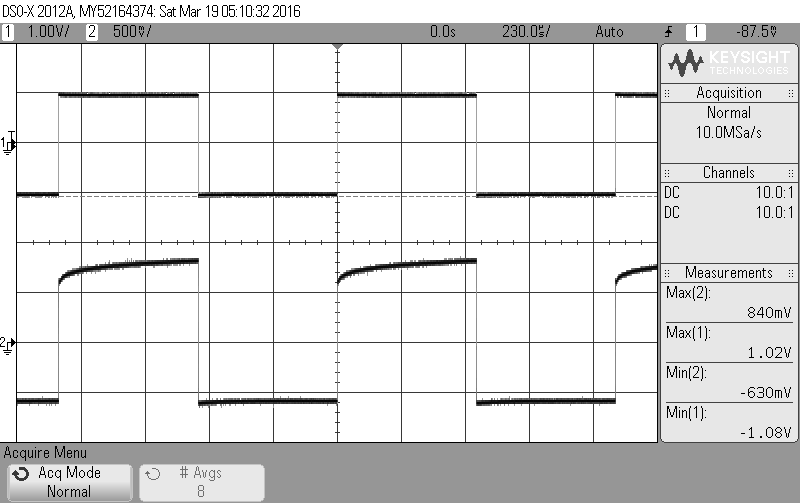
\includegraphics{response-first-order}
	\label{fig:first-order}
	\caption{Input and output of first order system with an integrator}
\end{figure}

\clearpage
